%%%%%%%%%%%%%%%%%%%%% {{{
%%Options for presentations (in-class) and handouts (e.g. print).
\documentclass[pdf,9pt]{beamer}
% \documentclass[pdf,9pt]{beamer}


%%%%%%%%%%%%%%%%%%%%%%
%Change this for different slides so it appears in bar
\usepackage{authoraftertitle}
\date{Chapter 2. Matrix Algebra \\ \S 2-2. Equations, Matrices, and Transformations}

%%%%%%%%%%%%%%%%%%%%%%
%% Upload common style file
\usepackage{LyryxLAWASlidesStyle}

\begin{document}

%%%%%%%%%%%%%%%%%%%%%%%
%% Title Page and Copyright Common to All Slides

%Title Page
\input frontmatter/titlepage.tex

%LOTS Page
\input frontmatter/lyryxopentexts.tex

%Copyright Page
\input frontmatter/copyright.tex

%%%%%%%%%%%%%%%%%%%%%%%%% }}}

%-------------- start slide -------------------------------%{{{ 2
\begin{frame}[fragile]
   \tableofcontents
\end{frame}
%-------------- end slide -------------------------------%}}}

\section[\textcolor{yellow}{}]{\textcolor{yellow}{Vectors}}

%-------------- start slide -------------------------------%{{{ 3
\frame{
\frametitle{Vectors}
\pause
\begin{definitions}
    A row matrix or column matrix is often called a
    \alert{vector}, and such matrices are referred to as
    \textcolor{yellow}{row vectors} and \textcolor{lgtblue}{column vectors},
    respectively.
    If $\vec{x}$ is a \textcolor{yellow}{row vector} of size $1\times n$, and
    $\vec{y}$ is a \textcolor{lgtblue}{column vector} of size $m\times 1$,
    then we write
    \[
	\vec{x}= \textcolor{yellow}{\left[\begin{array}{cccc} x_1 & x_2 & \cdots & x_n\end{array} \right]}
	\qquad\text{and}\qquad
	\vec{y}= \textcolor{lgtblue}{\left[\begin{array}{c} y_1 \\ y_2 \\ \vdots \\ y_m\end{array} \right]}
    \]
\end{definitions}
}

%-------------- end slide -------------------------------%}}}

%-------------- start slide -------------------------------%{{{ 4
\frame{
\begin{definition}[ Vector form of a system of linear equations ]
    Consider the system of linear equations
    \begin{equation*}
    \begin{array}{ccccccccc}
	a_{11}x_{1} & + & a_{12}x_2 & + & \cdots & + & a_{1n}x_{n} & = & b_{1}  \\
	a_{21}x_{1} & + & a_{22}x_2 & + & \cdots & + & a_{2n}x_{n} & = & b_{2}  \\
	 \vdots     &   & \vdots    &   &        &   & \vdots      &   & \vdots \\
	a_{m1}x_{1} & + & a_{m2}x_2 & + & \cdots & + & a_{mn}x_{n} & = & b_{m}
    \end{array}
    \end{equation*}
    \pause
    Such a system can be expressed in \alert{vector form}
    or as a \alert{vector equation} by using
    \textcolor{blue}{linear combinations} of column vectors:
    \[
	x_1 \left[ \begin{array}{c} a_{11}\\ a_{21}\\ \vdots \\ a_{m1} \end{array} \right] +
	x_2 \left[ \begin{array}{c} a_{12}\\ a_{22}\\ \vdots \\ a_{m2} \end{array} \right] + \cdots +
	x_n \left[ \begin{array}{c} a_{1n}\\ a_{2n}\\ \vdots \\ a_{mn} \end{array} \right]
    =
    \left[ \begin{array}{c} b_1\\ b_2\\ \vdots \\ b_m \end{array} \right]
    \]
\end{definition}
}
%-------------- end slide -------------------------------%}}}

%-------------- start slide -------------------------------%{{{ 5
\frame{
\begin{problem}
    Express the following system of linear equations in vector form:
    \[ \begin{array}{ccccccr}
	2x_1 & + & 4x_2 & - & 3x_3  & = & -6 \\
	     & - & x_2  & + & 5 x_3 & = & 0  \\
	x_1  & + & x_2  & + & 4x_3  & = & 1
    \end{array}\]
\end{problem}
\vfill
\pause
\begin{solution}
    \[
	x_1 \left[ \begin{array}{r} 2\\  0\\  1 \end{array} \right] +
	x_2 \left[ \begin{array}{r} 4\\  -1\\ 1 \end{array} \right] +
	x_3 \left[ \begin{array}{r} -3\\ 5\\  4 \end{array} \right]
    = \left[ \begin{array}{r} -6\\ 0\\ 1 \end{array} \right] \]
\end{solution}
}
%-------------- end slide -------------------------------%}}}

\section[\textcolor{yellow}{}]{\textcolor{yellow}{Matrix Vector Multiplication}}

%-------------- start slide -------------------------------%{{{ 6
\frame{
\frametitle{Matrix vector multiplication}
\pause
\begin{definition}
    Let $A=\left[ a_{ij} \right]$ be an $m\times n$ matrix with
    columns $\vec{a}_1, \vec{a}_2, \ldots, \vec{a}_n$, written
    $A= \left[ \begin{array}{cccc}
    \vec{a}_1 & \vec{a}_2 & \cdots &\vec{a}_n \end{array}\right]$,
    and let $\vec{x}$ be an $n\times 1$ column vector,
    \[ \vec{x} = \left[ \begin{array}{r} x_1 \\ x_2 \\ \vdots \\ x_n
    \end{array} \right] \]
    \pause
    Then \alert{the product of matrix $A$ and (column) vector $\vec{x}$}
    is the $m\times 1$ column vector given by
    \[
    \left[ \begin{array}{cccc}
    \vec{a}_1 & \vec{a}_2 & \cdots & \vec{a}_n \end{array}\right]
    \left[ \begin{array}{r} x_1 \\ x_2 \\ \vdots \\ x_n
    \end{array} \right] =
    x_{1}\vec{a}_{1}+x_{2}\vec{a}_{2}+\cdots +x_{n}\vec{a}_{n} = \sum_{j=1}^{n}x_{j}\vec{a}_{j}
    \]
    that is, $A\vec{x}$ is a \textcolor{blue}{linear combination} of the
    columns of $A$.
\end{definition}
}
%-------------- end slide -------------------------------%}}}

%-------------- start slide -------------------------------%{{{ 7
\frame{
\begin{problem}
    Compute the product $A\vec{x}$ for
    \[ A= \left[ \begin{array}{rr}
    1 & 4 \\ 5 & 0 \end{array} \right]\quad\text{and}\quad
    \vec{x}= \left[ \begin{array}{r} 2 \\ 3 \end{array} \right] \]
\end{problem}
\pause
\vfill
\begin{solution}
    \[ A\vec{x}=
    \left[ \begin{array}{rr} 1 & 4 \\ 5 & 0 \end{array} \right]
    \left[ \begin{array}{r} 2 \\ 3 \end{array} \right] =
    2 \left[ \begin{array}{r} 1 \\ 5 \end{array} \right]
    + 3 \left[ \begin{array}{r} 4 \\ 0 \end{array} \right]
    = \left[ \begin{array}{r} 2 \\ 10 \end{array} \right]
    + \left[ \begin{array}{r} 12 \\ 0 \end{array} \right]
    = \left[ \begin{array}{r} 14 \\ 10 \end{array} \right]
    \]
\end{solution}
}
%-------------- end slide -------------------------------%}}}

%-------------- start slide -------------------------------%{{{ 8
\frame{
\begin{problem}
    Compute $A\vec{y}$ for
    \[ A=\left[\begin{array}{rrrr}
	1 & 0  & 2 & -1 \\
	2 & -1 & 0 & 1  \\
	3 & 1  & 3 & 1
    \end{array}\right] \quad\text{and}\quad
    \vec{y}=\left[\begin{array}{r}
	2 \\ -1 \\ 1 \\ 4
    \end{array}\right]
    \]
\end{problem}
\pause
\vfill
\begin{solution}
    $A\vec{y} =
    2\left[\begin{array}{r}    1  \\ 2  \\ 3  \end{array}\right] +
    (-1)\left[\begin{array}{r} 0  \\ -1 \\ 1  \end{array}\right] +
    1\left[\begin{array}{r}    2  \\ 0  \\ 3  \end{array}\right] +
    4\left[\begin{array}{r}    -1 \\ 1  \\ 1  \end{array}\right] =
    \left[\begin{array}{r}     0  \\ 9  \\ 12 \end{array}\right]$
\end{solution}
}
%-------------- end slide -------------------------------%}}}

%-------------- start slide -------------------------------%{{{ 9
\frame{
\begin{definition}[ Matrix form of a system of linear equations ]
    Consider the system of linear equations
    \[ \begin{array}{ccccccccc}
	a_{11}x_{1} & + & a_{12}x_2 & + &  \cdots & + & a_{1n}x_{n} & = & b_{1} \\
	a_{21}x_{1} & + & a_{22}x_2 & + &  \cdots & + & a_{2n}x_{n} & = & b_{2} \\
	\vdots &  & \vdots & & & & & & \vdots \\
	a_{m1}x_{1} & + & a_{m2}x_2 & + &  \cdots & + & a_{mn}x_{n} & = & b_{m}
    \end{array}\]
    Such a system can be expressed in
    \alert{matrix form} using matrix vector multiplication,
    \[ \left[ \begin{array}{cccc}
	    a_{11} & a_{12} & \cdots & a_{1n} \\
	    a_{21} & a_{22} & \cdots & a_{2n} \\
	    \vdots & \vdots &        & \vdots \\
	    a_{m1} & a_{m2} & \cdots & a_{mn}
    \end{array} \right]
    \left[ \begin{array}{c} x_{1} \\ x_{2} \\ \vdots \\ x_{n}
    \end{array} \right]
    =
    \left[ \begin{array}{c} b_{1}\\ b_{2}\\ \vdots \\ b_{m}
    \end{array} \right] \]
    \pause
    \vfill
    Thus a system of linear equations can be expressed as a
    \alert{matrix equation $$A\vec{x}=\vec{b},$$}
    where \textcolor{blue}{$A$ is the coefficient matrix},
    \textcolor{blue}{$\vec{b}$ is the constant matrix}, and
    \textcolor{blue}{$\vec{x}$ is the matrix of variables.}
\end{definition}
}
%-------------- end slide -------------------------------%}}}

%-------------- start slide -------------------------------%{{{ 10
\frame{
\begin{problem}
Express the following system of linear equations in matrix form.
\[ \begin{array}{ccccccr}
    2x_1 & + & 4x_2 & - & 3x_3  & = & -6 \\
         & - & x_2  & + & 5 x_3 & = & 0  \\
    x_1  & + & x_2  & + & 4x_3  & = & 1
\end{array}\]
\end{problem}
\vfill
\pause
\begin{solution}
    \[ \left[ \begin{array}{rrr}
    2 & 4 & -3\\ 0 & -1 & 5\\ 1 & 1 & 4 \end{array} \right]
    \left[ \begin{array}{c} x_1 \\ x_2 \\ x_3 \end{array} \right]
    = \left[ \begin{array}{r} -6 \\ 0\\ 1 \end{array} \right]\]
\end{solution}
}
%-------------- end slide -------------------------------%}}}

%-------------- start slide -------------------------------%{{{ 11
\frame{
\begin{theorem}
\begin{enumerate}
    \item Every system of $m$ linear equations in $n$ variables can be written in the form $A\vec{x}=\vec{b}$ where $A$
	is the coefficient matrix, $\vec{x}$ is the matrix of variables, and $\vec{b}$ is the constant matrix.
\end{enumerate}
\end{theorem}
}
%-------------- end slide -------------------------------%}}}

%-------------- start slide -------------------------------%{{{ 12
\begin{frame}[fragile]
\begin{theorem}[continued]
\begin{enumerate}
    \item[2.] The system $A\vec{x}=\vec{b}$ is consistent (i.e., has at least one solution)
if and only if $\vec{b}$ is a linear combination of the columns of $A$.
\end{enumerate}
\end{theorem}
\end{frame}
%-------------- end slide -------------------------------%}}}

%-------------- start slide -------------------------------%{{{ 13
\begin{frame}[fragile]
\begin{theorem}[continued]
\begin{enumerate}
    \item[3.] The vector $\vec{x}=\left[ \begin{array}{c} x_1 \\ x_2 \\ \vdots \\ x_n \end{array}\right]$ is a solution
	to the system $A\vec{x}=\vec{b}$ if and only if $x_1, x_2, \ldots, x_n$ are a solution to the vector equation
	\[ x_1\vec{a}_1 + x_2\vec{a}_2 + \cdots x_n\vec{a}_n=\vec{b} \]
	where $\vec{a}_1, \vec{a}_2, \ldots, \vec{a}_n$ are the columns of $A$.
\end{enumerate}
\end{theorem}
\end{frame}
%-------------- end slide -------------------------------%}}}

%-------------- start slide -------------------------------%{{{ 14
\frame{
    \begin{problem}
	Let
	% \vspace*{-.3in}

	\[ A=\left[\begin{array}{rrrr}
		1 & 0 & 2 & -1 \\
		2 & -1 & 0 & 1 \\
		3 & 1 & 3 & 1
	\end{array}\right]
	\quad\text{and}\quad \vec{b} =\left[\begin{array}{r}
	1 \\ 1 \\ 1 \end{array}\right] \]

	Express $\vec{b}$ as a linear combination of the columns $\vec{a}_1, \vec{a}_2, \vec{a}_3, \vec{a}_4$ of $A$, or show that this is impossible.
    \end{problem}

}
%-------------- end slide -------------------------------%}}}

%-------------- start slide -------------------------------%{{{ 15
\begin{frame}[fragile]
    \begin{solution}
	Solve the system $A\vec{x}=\vec{b}$ where $\vec{x}$ is a column vector with
	four entries.
	\pause
	Do so by putting the {\bf augmented matrix}
	$\left[ \begin{array}{c|c} A & \vec{b} \end{array}\right]$
	in reduced row-echelon form.
	\pause

	\[ \left[\begin{array}{rrrr|r}
		1 & 0 & 2 & -1 & 1 \\
		2 & -1 & 0 & 1 & 1 \\
		3 & 1 & 3 & 1 & 1
	\end{array}\right]
	\rightarrow \cdots \rightarrow
	\left[\begin{array}{rrrr|r}
		1 & 0 & 0 & 1  & 1/7 \\
		0 & 1 & 0 & 1  & -5/7 \\
		0 & 0 & 1 & -1 & 3/7
	\end{array}\right]
    \]
    \pause
    Since there are infinitely many solutions ($x_4$ is assigned
    a parameter), choose any value for $x_4$.
    \pause
    Choosing $x_4=0$ (which is the simplest thing to do) gives us

    \[ \vec{b} = \left[\begin{array}{r} 1 \\ 1\\ 1 \end{array}\right]
    = \frac{1}{7} \left[\begin{array}{r} 1 \\ 2 \\ 3
    \end{array}\right]
    -\frac{5}{7}\left[\begin{array}{r} 0 \\ -1 \\ 1
    \end{array}\right] +
    \frac{3}{7}\left[\begin{array}{r} 2 \\ 0 \\ 3
    \end{array}\right]
    =\frac{1}{7} \vec{a}_{1} - \frac{5}{7} \vec{a}_{2} + \frac{3}{7} \vec{a}_{3} + 0 \vec{a}_{4}.\]
    \myQED
\end{solution}
\end{frame}
%-------------- end slide -------------------------------%}}}

%-------------- start slide -------------------------------%{{{ 16

\begin{frame}[fragile]
\begin{remark}
    The problem may ask to to find \alert{all possible} linear combinations of
    the columns $\vec{a}_1$, $\vec{a}_2$, $\vec{a}_3$, $\vec{a}_4$ of $A$.
    \vspace{1em}\pause

    This is equivalent to find all solutions to the corresponding system of
    linear equations:

    \begin{align*}
        \begin{bmatrix}
	    x_1\cr x_2	\cr x_3\cr x_4
	\end{bmatrix}
	=
	\begin{bmatrix}
	    \frac{1}{7}-s\\
	   -\frac{5}{7} - s \\
	    \frac{3}{7} +s \cr
	    s
	\end{bmatrix}
    \end{align*}
    \vspace{1em}\pause
    Hence, all possible linear combinations are:
    \begin{align*}
	\vec{b} =
	\left(\frac{1}{7}-s\right) \begin{bmatrix} 1\\ 2 \cr 3  \end{bmatrix}
	-\left(\frac{5}{7}+s\right) \begin{bmatrix} 0 \cr -1 \cr 1 \end{bmatrix}
	+\left(\frac{3}{7}+s\right) \begin{bmatrix} 2\cr 0 \cr 3 \end{bmatrix}
	+s \begin{bmatrix} -1 \cr 1 \cr 1 \end{bmatrix}
    \end{align*}
\end{remark}


\end{frame}
%-------------- end slide -------------------------------%}}}

%-------------- start slide -------------------------------%{{{ 17
\frame{
\begin{theorem}
    Let $A$ and $B$ be $m \times n$ matrices, and let $\vec{x}$ and $\vec{y}$ be n-vectors in $\RR^n$. Then:
    \begin{enumerate}
	\item $A(\vec{x}+\vec{y}) = A\vec{x}+A\vec{y}$.
	\item $A(a\vec{x}) = a(A\vec{x}) = (aA)\vec{x}$ for all scalars $a$.
	\item $(A+B)\vec{x} = A\vec{x}+B\vec{x}$.
    \end{enumerate}
\end{theorem}
\vfill
\pause
\begin{emptytitle}
    This provides a useful way to describe the solutions to a system $A\vec{x}=\vec{b}$.
    \bigskip

    {\noindent\bf Structure of solutions:}
    \bigskip
    \begin{center}
        General solution  = \textcolor{green}{Sol. to the Homog. Eq.} + \textcolor{red}{A Particular Solution}.
    \end{center}
    \bigskip
    \begin{align*}
       A \vec{x} = A \left(\vec{x}_0 + \vec{x}_1\right) = \underbrace{\textcolor{green}{A \vec{x}_0}}_{\text{$\vec{x}_0$: homogeneous sol.}} + \underbrace{ \textcolor{red}{A \vec{x}_1}}_{\text{$\vec{x}_1$: particular sol.}} = \textcolor{green}{\vec{0}} + \textcolor{red}{\vec{b}} = \vec{b}.
    \end{align*}
\end{emptytitle}
% \vfill
% \pause
% \begin{theorem}
%     Suppose $\vec{x}_{1}$ is any particular solution to the
%     system $A\vec{x} =\vec{b}$ of linear equations. Then every solution
%     $\vec{x}_{2}$ to $A\vec{x} =\vec{b}$ has the form $\vec{x}_{2}
%     =\vec{x}_{0}+\vec{x}_{1}$ for some solution $\vec{x}_{0}$ of the
%     associated homogeneous system $A\vec{x} =\vec{0}$.
% \end{theorem}

}
%-------------- end slide -------------------------------%}}}


\section[\textcolor{yellow}{}]{\textcolor{yellow}{The Dot Product}}

%-------------- start slide -------------------------------%{{{ 18
\frame{
\frametitle{The Dot Product}
\pause
\begin{definition}
    If $(a_1,a_2,\ldots,a_n)$ and $(b_1,b_2,\ldots,b_n)$ are two ordered n-tuples, their
    \alert{dot product} is defined to be the number
    \[ a_{1}b_{1} + a_{2}b_{2} + \dots + a_{n}b_{n} \]
    obtained by multiplying corresponding entries and adding the results.
\end{definition}
\vfill
\pause
\begin{emptytitle}
    This give an alternative way to carry out the matrix-vector product $A \vec{x}$.
\end{emptytitle}
\vfill

% \begin{theorem}[ Dot Product Rule ]
%     Let $A$ be an $m \times n$ matrix and let  $\vec{x}$ be an n-vector.
%     Then each entry of the vector $A\vec{x}$ is the dot product of the corresponding row of $A$ with
%     $\vec{x}$.
% \end{theorem}
\begin{equation*}
\leftB\begin{array}{ccc}
   \;          & \tn{A}{}    & \;           \\
  \tn{rowi1}{} & \tn{rowi}{} & \tn{rowi2}{} \\
               &             &              \\
\end{array}\rightB
\leftB\begin{array}{c}
  \tn{columnx1}{}\\
   \\
  \tn{columnx2}{} \\
\end{array}\rightB =
\leftB \begin{array}{c}
  \\
  \tn{ientry}{} \\
  \\
\end{array}\rightB
\end{equation*}
\begin{tikzpicture}[remember picture, overlay]
  \draw[color=blue!30!gray,opacity=0.3,line width=4mm, line cap=round](rowi1.west) --(rowi2.east);
  \draw[-latex](rowi1)--(rowi2);
  \draw[color=blue!30!gray,opacity=0.3,line width=4mm, line cap=round,shorten >=0.1cm](columnx1.north) -- (columnx2);
  \draw[-latex](columnx1)--(columnx2);
  \draw[color=blue!30!gray,opacity=0.3,line width=4mm, line cap=round](ientry.west) -- (ientry.east);
  \node[below =0.75cm of rowi, font=\footnotesize] (rowlabel){row $i$};
  \draw[thin] (rowi.south)++(0,-0.1cm) to [bend right] (rowlabel.north);
  \node[below=0.75cm of ientry, font=\footnotesize] (ijlabel){entry $i$};
  \draw[thin] (ientry.south)++(0,-0.05cm) to [bend left] (ijlabel.north);
  \node[above=0.35cm of A, font=\footnotesize]{$A$};
  \node[above=0.35cm of columnx1, font=\footnotesize]{$\vec{x}$};
  \node[above=0.85cm of ientry, font=\footnotesize]{$A\vec{x}$};
\end{tikzpicture}
}
%-------------- end slide -------------------------------%}}}

%-------------- start slide -------------------------------%{{{ 1
\begin{frame}[fragile]
\begin{gather*}
A\vec{x}
\\ || \\
\leftB \begin{array}{cccc}
  a_{11} & a_{12} & a_{13} & a_{14} \\
  a_{21} & a_{22} & a_{23} & a_{24} \\
  a_{31} & a_{32} & a_{33} & a_{34}
\end{array} \rightB \leftB \begin{array}{c}
  x_{1} \\
  x_{2} \\
  x_{3} \\
  x_{4}
\end{array} \rightB
\\ || \\
\end{gather*}
\vspace{-3em}
\begin{align}
x_{1} \leftB \begin{array}{c}
  a_{11} \\
  a_{21} \\
  a_{31}
\end{array} \rightB + x_{2} \leftB \begin{array}{c}
  a_{12} \\
  a_{22} \\
  a_{32}
\end{array} \rightB + x_{3} \leftB \begin{array}{c}
  a_{13} \\
  a_{23} \\
  a_{33}
\end{array} \rightB + x_{4} \leftB \begin{array}{c}
  a_{14} \\
  a_{24} \\
  a_{34}
\end{array} \rightB
\tag{Def.}
\end{align}
\vspace{-3em}
\begin{align*}
\\ || \\
\end{align*}
\vspace{-3em}
\begin{align}
    \tag{Alternative}
    \leftB \begin{array}{c}
  a_{11}x_{1} + a_{12}x_{2} + a_{13}x_{3} + a_{14}x_{4} \\
  a_{21}x_{1} + a_{22}x_{2} + a_{23}x_{3} + a_{24}x_{4} \\
  a_{31}x_{1} + a_{32}x_{2} + a_{33}x_{3} + a_{34}x_{4}
\end{array} \rightB
\end{align}
\end{frame}
%-------------- end slide -------------------------------%}}}

%-------------- start slide -------------------------------%{{{ 19
\frame{
\begin{problem}
    If $A = \leftB \begin{array}{rrrr}
	1 & 0  & 2 & -1 \\
	2 & -1 & 0 & 1  \\
	3 & 1  & 3 & 1
    \end{array} \rightB$
    and $\vec{x} = \leftB \begin{array}{r}
	2 \\
	-1 \\
	1 \\
	4
    \end{array} \rightB,$
    compute $A \vec{x}$.
\end{problem}
\vfill
\pause
\begin{solution}
    The entries of $A \vec{x}$  are the dot products of the rows of $A$ with $\vec{x}$:
    $$\begin{array}{ll}
	A\vec{x} & =
	\leftB \begin{array}{rrrr}
	    1 & 0  & 2 & -1 \\
	    2 & -1 & 0 & 1  \\
	    3 & 1  & 3 & 1
	\end{array} \rightB
	\leftB \begin{array}{r}
	    2 \\
	    -1 \\
	    1 \\
	    4
	\end{array} \rightB \\
		 & = \leftB \begin{array}{rrrrrrr}
		     1 \cdot 2 & + & 0 (-1)   & + & 2 \cdot 1 & + & (-1)4 \\
		     2 \cdot 2 & + & (-1)(-1) & + & 0\cdot 1  & + & 1\cdot 4 \\
		     3\cdot 2  & + & 1(-1)    & + & 3 \cdot 1 & + & 1\cdot  4
		     \end{array} \rightB = \leftB \begin{array}{r}
		     0 \\
		     9 \\
		     12
		 \end{array} \rightB.
    \end{array}$$

    Of course, this agrees with the outcome of the previous example.
    \myQED
\end{solution}
}
%-------------- end slide -------------------------------%}}}

%-------------- start slide -------------------------------%{{{ 20
\frame{

\begin{definition}[ Identity Matrix ]
    For each $n > 2$, the \alert{identity matrix} $I_n$ is the $n \times n$ matrix with 1's on the
    main diagonal (upper left to lower right), and zeros elsewhere.
\end{definition}
\pause
\vfill
\begin{example}
    The first few identity matrices are
    \begin{equation*}
    I_{2} = \leftB \begin{array}{rr}
	1 & 0 \\
	0 & 1
    \end{array} \rightB, \quad I_{3} = \leftB \begin{array}{rrr}
	1 & 0 & 0 \\
	0 & 1 & 0 \\
	0 & 0 & 1
    \end{array} \rightB, \quad I_{4} = \leftB \begin{array}{rrrr}
	1 & 0 & 0 & 0 \\
	0 & 1 & 0 & 0 \\
	0 & 0 & 1 & 0 \\
	0 & 0 & 0 & 1
    \end{array} \rightB, \quad \dots
    \end{equation*}
\end{example}
}
%-------------- end slide -------------------------------%}}}

%-------------- start slide -------------------------------%{{{ 21
\frame{
\begin{problem}
    Show that $I_n \vec{x}=\vec{x}$  for each n-vector $\vec{x}$ in $\RR^n$, $n\ge 1$.
\end{problem}
\vfill
\pause
\begin{solution}
      We verify the case \textit{n} = 4. Given the 4-vector
      $\vec{x} = \leftB \begin{array}{c}
	  x_{1} \\
	  x_{2} \\
	  x_{3} \\
	  x_{4}
      \end{array} \rightB$  the dot product rule gives
      \begin{equation*}
	  I_{4}\vec{x} = \leftB \begin{array}{rrrr}
	      1 & 0 & 0 & 0 \\
	      0 & 1 & 0 & 0 \\
	      0 & 0 & 1 & 0 \\
	      0 & 0 & 0 & 1
	      \end{array} \rightB \leftB \begin{array}{c}
	      x_{1} \\
	      x_{2} \\
	      x_{3} \\
	      x_{4}
	      \end{array} \rightB = \leftB \begin{array}{c}
	      x_{1} + 0 + 0 + 0 \\
	      0 + x_{2} + 0 + 0 \\
	      0 + 0 + x_{3} + 0 \\
	      0 + 0 + 0 + x_{4}
	      \end{array} \rightB = \leftB \begin{array}{c}
	      x_{1} \\
	      x_{2} \\
	      x_{3} \\
	      x_{4}
	  \end{array} \rightB = \vec{x}.
      \end{equation*}\\

    In general, $I_n \vec{x}=\vec{x}$  because entry $k$  of $I_n \vec{x}$ is the dot product of row
    $k$ of $I_n$ with $\vec{x}$, and row $k$  of $I_n$ has 1 in position $k$  and zeros elsewhere.
    \myQED
\end{solution}
}


%-------------- end slide -------------------------------%}}}

\section[\textcolor{yellow}{}]{\textcolor{yellow}{Transformations}}

%-------------- start slide -------------------------------%{{{ 22
\frame{
\frametitle{Transformations}
\pause
\begin{block}{Notation and Terminology}
    \pause
    \begin{itemize}
	\item We have already used \alert{$\RR$} to denote the set of \alert{real numbers}.  \pause
	\item We use \alert{$\RR^2$} to the denote the set of all \alert{column vectors of length two},
	    \pause
	     and we use
	    \alert{$\RR^3$} to the denote the set of
	    all \alert{column vectors of length three}
	    \pause
	    \textcolor{blue}{(the length of a vector is the number
	    of entries it contains).}
	    \pause
	\item In general, we write \alert{$\RR^n$} for the set of all \alert{column vectors of length $n$}.
    \end{itemize}
\end{block}
\pause
\vfill
\begin{alertblock}{$\RR^2$ and $\RR^3$}
    Vectors in $\RR^2$ and $\RR^3$ have convenient geometric
    interpretations as {\bf position vectors} of points in
    the 2-dimensional (Cartesian) plane and in 3-dimensional
    space, respectively.
\end{alertblock}
}
%-------------- end slide -------------------------------%}}}

%-------------- start slide -------------------------------%{{{ 23
\begin{frame}[fragile]
    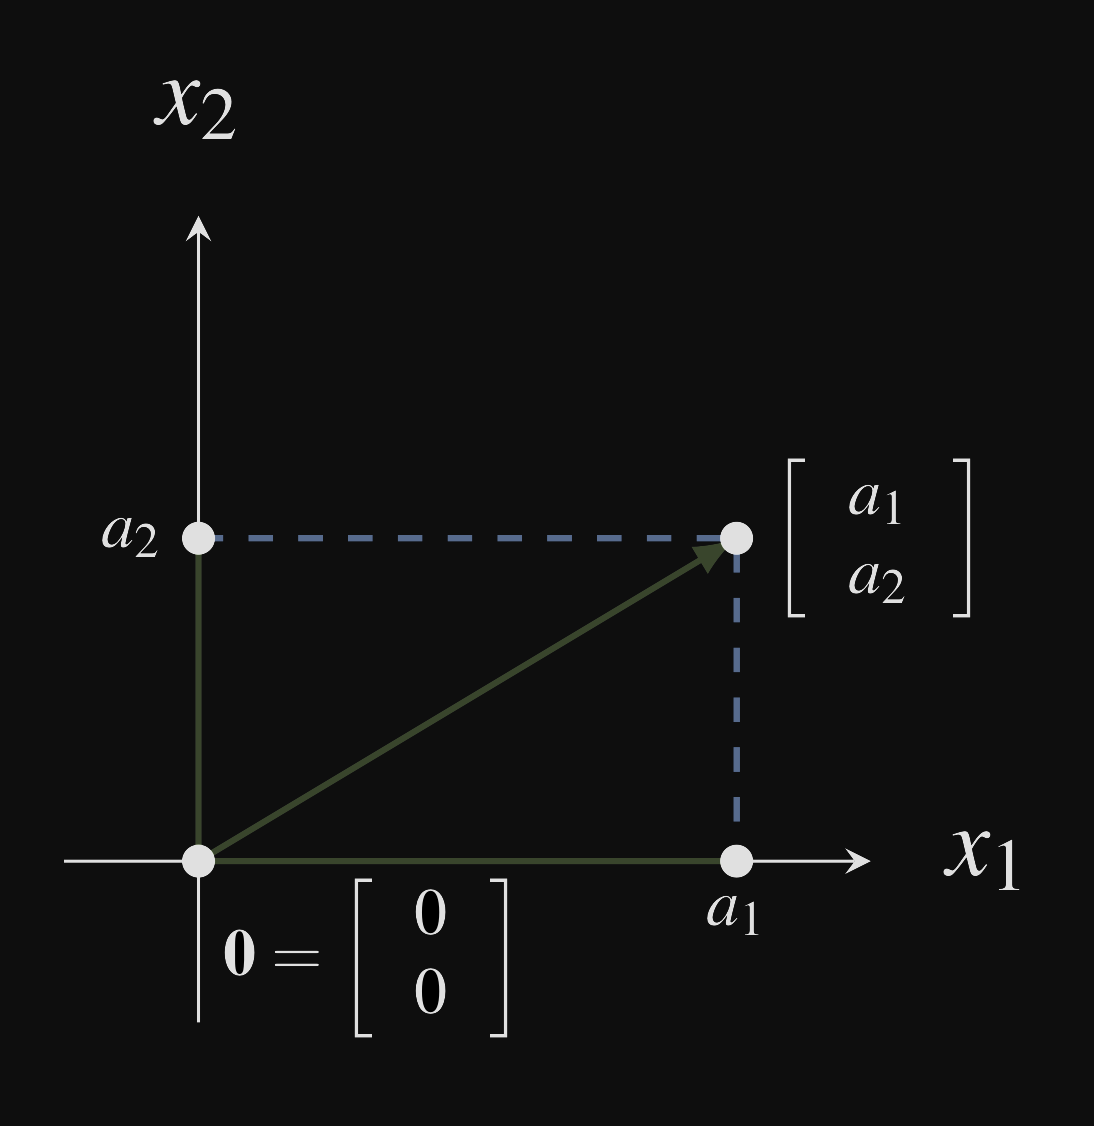
\includegraphics[scale=0.11]{R2.png}
    \hfill
    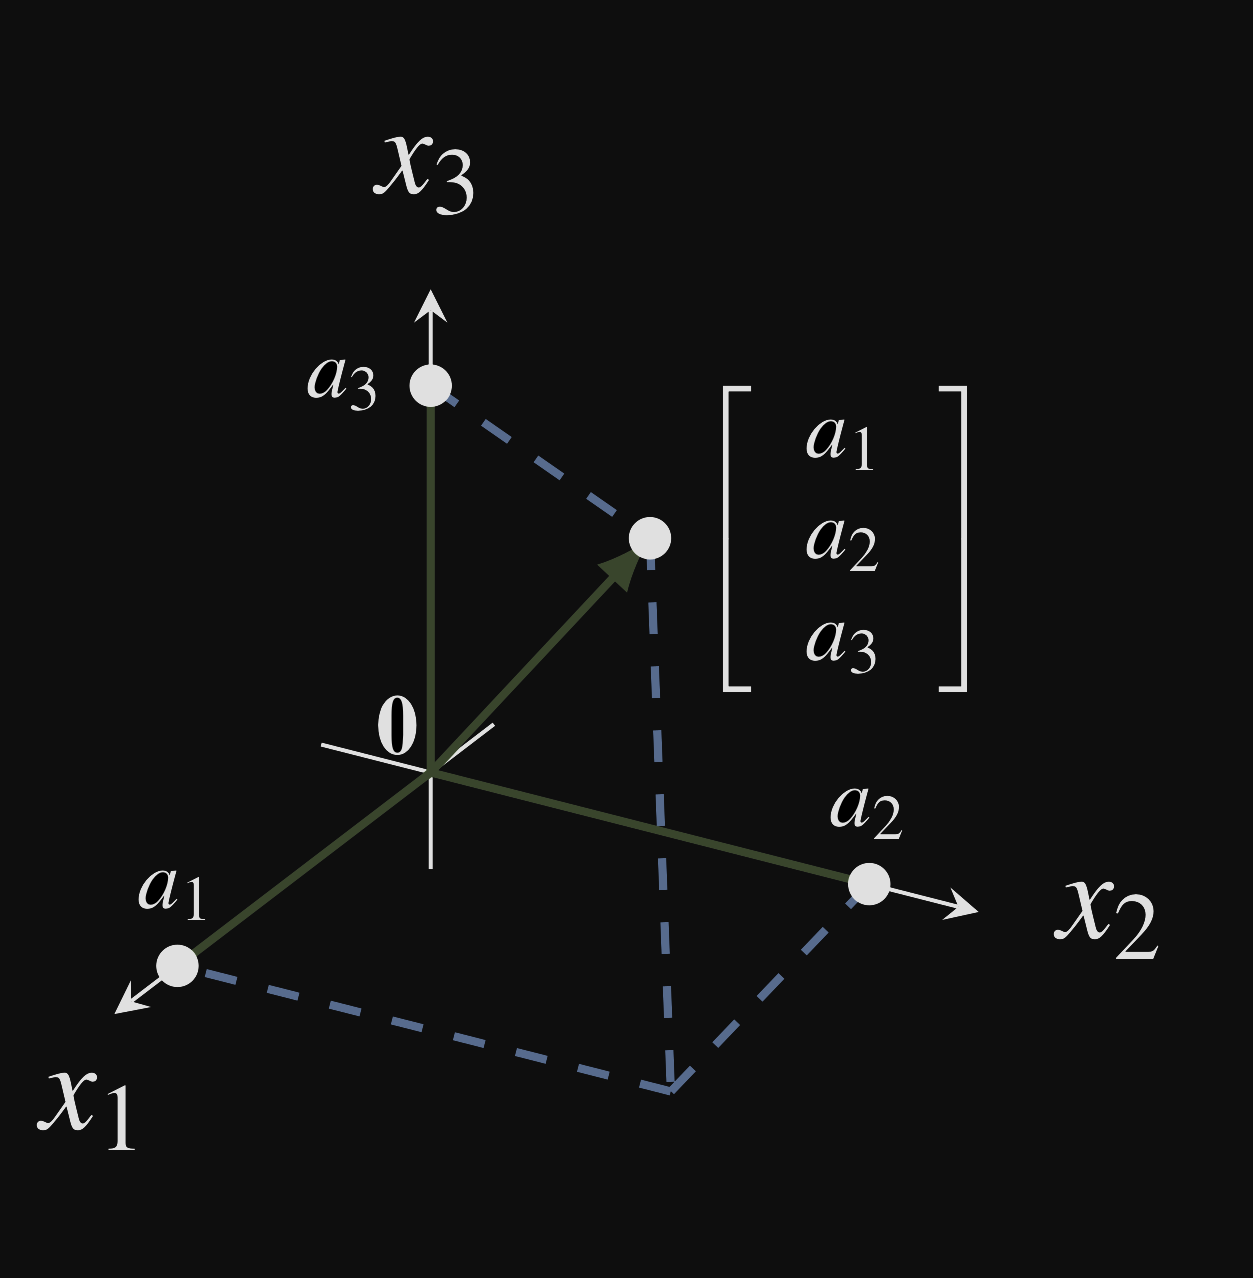
\includegraphics[scale=0.1]{R3.png}
\end{frame}
%-------------- end slide -------------------------------%}}}

%-------------- start slide -------------------------------%{{{ 24
\frame{
\begin{definition}[Transformations]
    A \alert{transformation} is a function $T:\RR^n\rightarrow \RR^m$, sometimes written
    $\RR^n\stackrel{T}{\rightarrow} \RR^m$, and is called a \alert{transformation from $\RR^n$ to
    $\RR^m$}.
    \pause
    If $m=n$, then we say \alert{$T$ is a transformation of $\RR^n$.}
\end{definition}
\vfill
\pause
\begin{block}{What do we mean by a function?}
    \pause
    Informally, a function $T:\RR^n\to\RR^m$ is a rule that, for each vector in
    $\RR^n$, assigns exactly one vector of $\RR^m$ \\[1em]
    We use the notation $T(\vec{x})$ to mean the transformation $T$ applied to the vector $\vec{x}$.
\end{block}
\pause
\vfill
\begin{definition}
    If $T$ acts by matrix multiplication of a matrix $A$ (such as the previous example), we call $T$
    a \alert{matrix transformation}, and write $T_A(\vec{x}) = A\vec{x}$.
\end{definition}
}


%-------------- end slide -------------------------------%}}}

%-------------- start slide -------------------------------%{{{ 25
\frame{
\begin{definition}[ Equality of Transformations ]
    Suppose $S:\RR^n\rightarrow\RR^m$ and $T:\RR^n\rightarrow\RR^m$ are transformations.
    Then \textcolor{red}{$S=T$} if and only if $S(\vec{x})=T(\vec{x})$ for every $\vec{x}\in\RR^n$.
\end{definition}
}
%-------------- end slide -------------------------------%}}}

%-------------- start slide -------------------------------%{{{ 26
\frame{
\begin{example}[ Specifying the action of a transformation ]
    $T:\RR^3\rightarrow\RR^4$ defined by
    \[
	T\left[\begin{array}{c} a \\ b\\ c\end{array}\right]
	=\left[ \begin{array}{c}
	a+b \\ b+c \\ a-c\\ c-b \end{array}\right]
    \]
    is a transformation
    \pause
    that \alert{transforms} the vector $\left[ \begin{array}{r}
	    1 \\ 4 \\ 7
	\end{array}
    \right]$ in $\RR^3$
    into the vector
    \[
	T\left[\begin{array}{r} 1 \\ 4\\ 7\end{array}\right]
	=\left[ \begin{array}{r}
	1 + 4 \\ 4+7 \\ 1-7\\ 7-4 \end{array}\right]
	=\left[ \begin{array}{r}
	5 \\ 11 \\ -6 \\ 3 \end{array}\right].
    \]
\end{example}
}
%-------------- end slide -------------------------------%}}}

%-------------- start slide -------------------------------%{{{ 27
\frame{
\begin{example}[ Transformation by matrix multiplication ]
    Consider the matrix $A = \left[
    \begin{array}{rrr}
	1 & 2 & 0 \\
	2 & 1 & 0
    \end{array}
    \right]$. By matrix multiplication, $A$ transforms vectors in $\mathbb{R}^3$ into vectors in $\mathbb{R}^2$.
    \pause
    Consider the vector $\left[
    \begin{array}{c}
    x \\
    y \\
    z
    \end{array}
    \right]$. \pause Transforming this vector by $A$ looks like:
    \[
    \left[
    \begin{array}{rrr}
	1 & 2 & 0 \\
	2 & 1 & 0
    \end{array}
    \right]
    \left[
    \begin{array}{c}
	x \\
	y \\
	z
    \end{array}
    \right]
    =
    \left[
    \begin{array}{c}
	x + 2y \\
	2x + y
    \end{array}
    \right].
    \]
    \pause

    For example:
    \[
    \left[
    \begin{array}{rrr}
	1 & 2 & 0 \\
	2 & 1 & 0
    \end{array}
    \right]
    \left[
    \begin{array}{c}
	1 \\
	2 \\
	3
    \end{array}
    \right]
    =
    \left[
    \begin{array}{c}
	5 \\
	4
    \end{array}
    \right].
    \]
\end{example}
}
%-------------- end slide -------------------------------%}}}

\section[\textcolor{yellow}{}]{\textcolor{yellow}{Rotations in $\mathbb{R}^2$}}

%-------------- start slide -------------------------------%{{{ 28
\frame{
\frametitle{Rotations in $\mathbb{R}^2$}
\pause
\begin{definition}
    Let $A$ be an $m\times n$ matrix.  The transformation
    $T:\RR^n\rightarrow\RR^m$ defined by
    \[ T(\vec{x})=A\vec{x} \mbox{ for each } \vec{x}\in\RR^n\]
    is called the
    \alert{matrix transformation induced by $A$}.
\end{definition}
\vfill
\pause
\begin{definition}
    The transformation
    \[ R_\theta: \RR^2\rightarrow \RR^2 \] denotes
    \textcolor{red}{counterclockwise rotation} about the origin through an angle of $\theta$.
\end{definition}
}
%-------------- end slide -------------------------------%}}}

%-------------- start slide -------------------------------%{{{ 29
\frame{
\begin{example}[Rotation through $\pi$]
    % \textcolor{titletextcolour}{Example (Rotation through $\pi$)}\\[0.5em]
    We denote by
    \[ R_{\pi}:\RR^2\to\RR^2\]
    counterclockwise rotation about the origin through an angle
    of $\pi$.
    \pause
    % \vspace{1em}
    \begin{center}
	    \begin{tikzpicture}[scale=1, transform shape]
	    \tikzset{>=latex}
	    \coordinate (P) at (1.25,1);
	    \coordinate (Q) at (-1.25,-1);
	    \coordinate (0) at (0,0);
	    % \draw (P) -- coordinate[pos={1/3}] (A) coordinate[pos={2/3}] (B) (Q) node [right] {$Q$};
	    % \draw [->,dashed] (0) node [below] {$} -- (P) node [above] {$P$};
	    \draw [->] (-2.3,0) -- (2.3,0) node [right] {$x$};
	    \draw [->] (0,-1.3) -- (0,1.3) node [above] {$y$};
	    \filldraw (0) circle (0.05);
	    \pause
	    \filldraw [blue] (P) circle (0.05);
	    \draw [->,blue] (0) -- (P) node [right] {$(a,b)$};
	    \pause
	    \draw [->,red] (0) -- (Q) node [left] {\textcolor{red}{$(-a,-b)$}};
	    \filldraw[red] (Q) circle (0.05);
	    \end{tikzpicture}
    \end{center}
    %
    % \begin{picture}(4,1.75)
    % \put(1.3,0.1){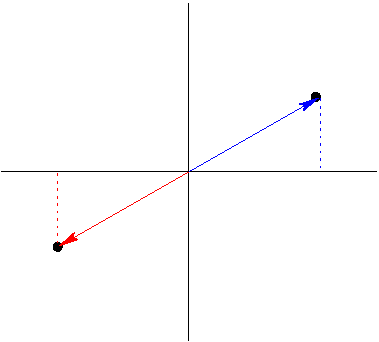
\includegraphics[scale=0.7]{figures/R2-rotate-pi.pdf}}
    % \put(2.25,0.75){\scriptsize{$0$}}
    % \put(2.05,1.6){\scriptsize{$y$}}
    % \put(3.0,0.75){\scriptsize{$x$}}
    % \put(2.85,1.22){\scriptsize{$(a,b)$}}
    % \pause
    % \put(1.0,0.5){\scriptsize{\alert{$(-a,-b)$}} }
    % \end{picture}
    \pause
    % \vspace{1em}
    \only<5->{
    We see that $ R_{\pi}\left[\begin{array}{c} a \\ b \end{array}\right]
    =
    \left[\begin{array}{c} -a \\ -b \end{array}\right]
    =
    \pause\left[\begin{array}{rr} -1 & 0 \\ 0 & -1 \end{array}\right]
    \left[\begin{array}{c} a \\ b \end{array}\right],$
    so $R_{\pi}$ is a matrix transformation.
    }
\end{example}
}
%-------------- end slide -------------------------------%}}}

%-------------- start slide -------------------------------%{{{ 30
\frame{
\begin{example}[Rotation through $\pi/2$]
    % \textcolor{titletextcolour}{Example (Rotation through $\pi/2$)}\\[0.5em]
    We denote by
    \[ R_{\pi/2}:\RR^2\to\RR^2\]
    counterclockwise rotation about the origin through an angle
    of $\pi/2$.
    % \vspace{1em}
    \pause
    \begin{center}
	    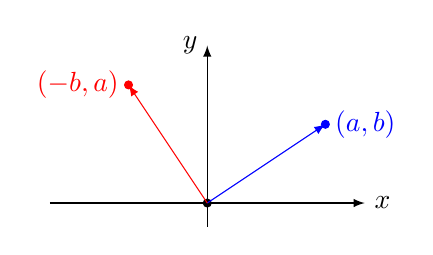
\begin{tikzpicture}[scale=1, transform shape]
	    \tikzset{>=latex}
	    \coordinate (P) at (1.5,1);
	    \coordinate (Q) at (-1,1.5);
	    \coordinate (0) at (0,0);
	    % \draw (P) -- coordinate[pos={1/3}] (A) coordinate[pos={2/3}] (B) (Q) node [right] {$Q$};
	    % \draw [->,dashed] (0) node [below] {$} -- (P) node [above] {$P$};
	    \draw [->] (-2,0) -- (2,0) node [right] {$x$};
	    \draw [->] (0,-0.3) -- (0,2) node [left] {$y$};
	    \filldraw (0) circle (0.05);
	    \pause
	    \filldraw [blue] (P) circle (0.05);
	    \draw [->,blue] (0) -- (P) node [right] {$(a,b)$};
	    \pause
	    \draw [->,red] (0) -- (Q) node [left] {\textcolor{red}{$(-b,a)$}};
	    \filldraw[red] (Q) circle (0.05);
	    \end{tikzpicture}
    \end{center}
    \pause
    % \vspace{1em}
    % \begin{picture}(4,1.75)
    % \put(1.3,0.1){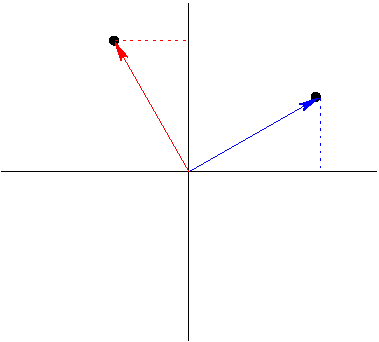
\includegraphics[scale=0.7]{figures/R2-rotate-halfpi.pdf}}
    % \put(2.25,0.75){\scriptsize{$0$}}
    % \put(2.05,1.6){\scriptsize{$y$}}
    % \put(3.0,0.75){\scriptsize{$x$}}
    % \put(2.85,1.22){\scriptsize{$(a,b)$}}
    % \pause
    % \put(1.4,1.5){\scriptsize{\alert{$(-b,a)$}} }
    % \end{picture}
    % \pause
    \only<5->{
    We see that $ R_{\pi/2}\left[\begin{array}{c} a \\ b \end{array}\right]
    =
    \left[\begin{array}{c} -b \\ a \end{array}\right]
    =
    \pause\left[\begin{array}{rr} 0 & -1 \\ 1 & 0 \end{array}\right]
    \left[\begin{array}{c} a \\ b \end{array}\right],$
    so $R_{\pi/2}$ is a matrix transformation.}
\end{example}
}
%-------------- end slide -------------------------------%}}}

%-------------- start slide -------------------------------%{{{ 31
\begin{frame}[fragile]
\begin{remark}
    In general, the rotation (counterclockwise) about the origin for an angle
    $\theta$ is
    \begin{align*}
	R_\theta =
	\begin{bmatrix} \cos(\theta) & -\sin(\theta)\cr
	\sin(\theta) & \cos(\theta) \end{bmatrix}
    \end{align*}
    and
    \pause
    \begin{align*}
        \begin{bmatrix} a'\cr b'\end{bmatrix}  =
	\begin{bmatrix} \cos(\theta) & -\sin(\theta)\cr
	\sin(\theta) & \cos(\theta) \end{bmatrix}
        \begin{bmatrix} a\cr b\end{bmatrix}
	=
	\begin{bmatrix} a\cos\left(\theta\right) - b\sin(\theta) \cr a
	\sin(\theta) + b\cos(\theta) \end{bmatrix}
    \end{align*}
    \pause
    \vspace{1em}
    \begin{align*}
	R_{\pi}   = \begin{bmatrix} -1&0\cr 0& -1  \end{bmatrix} \quad\text{and}\quad
	R_{\pi/2} = \begin{bmatrix} 0&-1\cr 1& 0  \end{bmatrix}
    \end{align*}
\end{remark}
\end{frame}
%-------------- end slide -------------------------------%}}}

\end{document}
